\chapter{Теоретический раздел}

\section{Равномерное распределение}
    
Говорят, что случайная величина $X$ имеет равномерное распределение на отрезке $[a,b]$, если её функция плотности имеет вид:

\begin{equation}
    f (x) =
    \begin{cases}
        \frac{1}{b-a}, x \in [a,b] \\
        0, x \notin [a, b] \\
    \end{cases}
\end{equation}

\begin{figure}[H]
    \begin{center}
    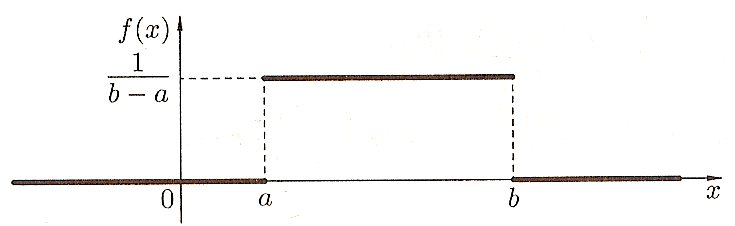
\includegraphics[width=0.5\linewidth]{inc/uni_f.png}
    \caption{Функция плотности равномерного распределения}
    \label{fig:}
    \end{center}
\end{figure}

Функция распределения:

\begin{equation}
F (x) =
    \begin{cases}
        0, x < a \\
        \frac{x - a}{b - a}, a \le x < b \\
        1, x \geq b \\
    \end{cases}
\end{equation}

\begin{figure}[H]
    \begin{center}
    \includegraphics[width=0.5\linewidth]{inc/uni_Fx.png}
    \caption{Функция распределения равномерного распределения}
    \label{fig:}
    \end{center}
\end{figure}

\section{Гиперэкспоненциальное распределение}

Говорят, что случайная величина $X$ имеет равномерное распределение на отрезке $[a,b]$, если её функция плотности имеет вид:

\begin{equation}
    f (x) = \sum_{i=1}^{n} f_{Y_i}(y) \cdot p_i = \sum_{i=1}^{n} p_i \cdot \lambda_i \cdot e^{-\lambda x},
\end{equation}

\noindent где $Y_i$~---~случайные величины, распределенные по экспоненциальному закону, $p_i$~---~вероятность того, что случайная величина $X$ пример значение $Y_i$, $\lambda_i$~---~коэффициент соответствующего экспоненциального распределения.

\begin{figure}[H]
    \begin{center}
    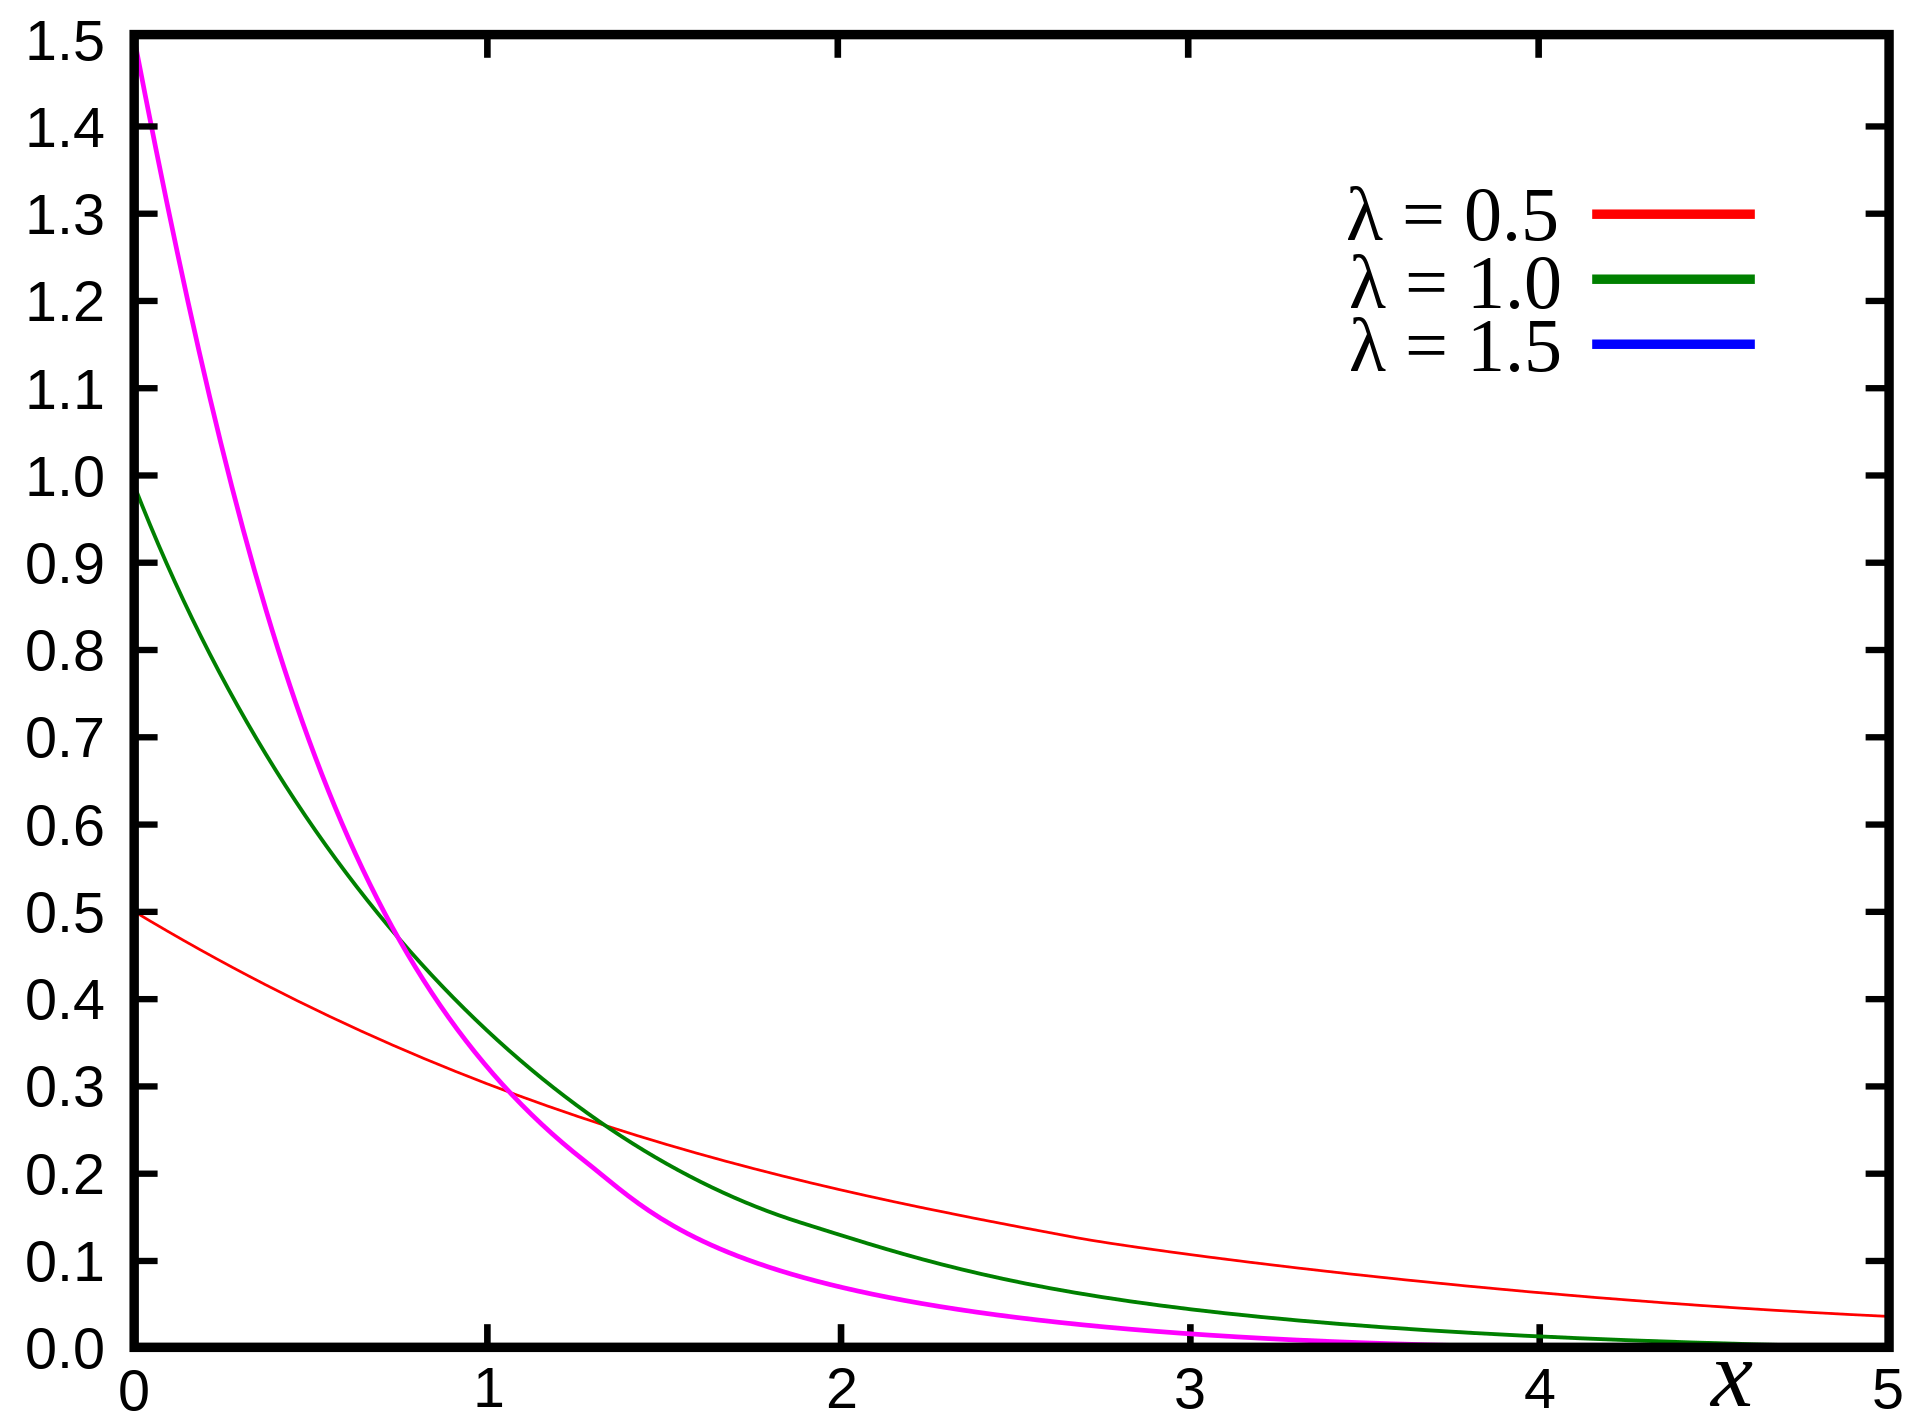
\includegraphics[width=0.5\linewidth]{inc/hyp_f.png}
    \caption{Функция плотности гиперэкспоненциального распределения}
    \label{fig:}
    \end{center}
\end{figure}

\newpage

Функция распределения:

\begin{equation}
F (x) = 1 - \sum_{i=1}^{n} p_i \cdot \cdot e^{-\lambda x}.
\end{equation}

\begin{figure}[H]
    \begin{center}
    \includegraphics[width=0.5\linewidth]{inc/hyp_Fx.png}
    \caption{Функция распределения гиперэкспоненциального распределения}
    \label{fig:}
    \end{center}
\end{figure}
